\documentclass[14pt,a4paper]{scrartcl}
\usepackage[utf8]{inputenc}
\usepackage{amsmath, amssymb, amsfonts}
\usepackage{graphicx}
\usepackage[top=3cm, bottom=2.5cm, left=3cm, right=4cm]{geometry}\usepackage[english,german]{babel} 
\usepackage{csquotes}

\usepackage[style=ieee]{biblatex}
 
 \graphicspath{ {./media/} } 
\parindent 0px
\linespread{1.25} %gleich wie 1.5 in word
\pagestyle{headings}

\addbibresource{ref.bib}

\begin{document} \selectlanguage{german}
\begin{titlepage}
 
  \null\vfill
  \begin{center}
    GYMNASIUM OTTOBRUNN
    \vskip 2em
    Oberstufenjahrgang 2022/2023
    \vskip 2em
    Seminar: Die Welt der Mathematik - die Mathematik in der Welt
    \vskip 1em
    Leitfach: Mathematik
    
    \vskip 5em
    Exposé zur Seminararbeit
    \vskip 2em
    
    {
      \usekomafont{title} \LARGE
        Der RSA - Algorithmus und seine Anwendung in der IT-Sicherheit
      \par
    }
     
    \vskip 1.5em
    {\usekomafont{date}{\today \par}}%
    \vskip 0pt plus 4fill
    
  \end{center}
  Verfasser: Julian Thanner
  \vskip 0.5em
  Seminarleiterin: StDin Birgit Gregor
  \vskip 2em
  Bewertung: .............. Punkte
  \vskip 1em
  Unterschrift der Seminarleiterin: \underline{\hspace{5cm}}
 \end{titlepage}
	
\thispagestyle{empty}
\tableofcontents
\thispagestyle{empty}


\pagebreak
\section{Einleitung}
\subsection{Heutige Sicherheit im Internet}
Eigentlich ist es doch sehr erstaunlich, dass wir unser Geld einfach so über unser Handy verwalten können und keine Sorge haben müssen, dass jemand fremdes unerlaubt Dinge mit unserem Geld anstellt. Oder das wir einfach mal eben eine Nachricht an jemanden schicken können, ohne uns Gedanken machen zu müssen, dass jemand fremdes diese Nachrichten mitlesen kann. Wenn man sich überlegt, dass wir und die andere Seite nichts gemeines teilen, wenn wir die Person nicht kennen, wie z.B. einen Schlüssel für ein Schloss. Und auch die Zwischenpartei ist dabei nur mittelmäßig hilfreich, da wir mit dieser ja bei der ersten Benutzung auch nichts gemeinsames Teilen. Dieses Problem wird durch die asymmetrische Verschlüsselung gelöst.
\subsection{Nachteile der symmetrischen Verschlüsselung}

Bei symmetrischen Verschlüsselungsverfahren gibt es, anders als bei asymmetrischen Verfahren (auch: Public Key Verfahren), nur einen Schlüssel für die Ent- und Verschlüsselung. Das Problem hierbei ist allerdings, sie sind nur dann sicher, wenn es möglich ist den Schlüssel sicher der anderen Seite zukommen zu lassen. In der Praxis ist das aber nur mit einem persönlichen Treffen möglich. Wenn man aber eine E-Mail an jemanden schicken möchte, mit dem man sich aktuell nicht physisch treffen kann, ist ein Schlüsselaustausch so nicht möglich.

\section*{Zeitplan}

%beginn ende was 
	\begin{tabular}{ c | c | p{10cm} }
	Beginn & Ende & Aufgabe\\
	 \hline

 & 14.6 & Expose abgegeben \\
14.6 & 28.6 & Vorbereitungen machen, wie Begriffserklärungen schreiben \\
28.6 & 28.7 & Fertig schreiben der Seminar Arbeit, da sonst wenig Zeit \\
28.8 & 17.9 & Korrektur lesen und Fehler korrigieren\\
18.9 & 20.10 & Puffer/Alles druckbereit und keine Fehler mehr\\
21.10 & 27.10 & Alles fertig und gedruckt
	\end{tabular}
	
	

\section{Begriffserklärungen}
	\subsection{Modulo Operation} %Notwendigkeit?
	\subsection{Einwegverschlüsselungsverfahren}
	\label{ch:einweg}
	\subsection{Eulersche $\phi$ Funktion}
	\subsection{Satz von Euler}
	\subsection{Der euklidische Algorithmus}
	\subsection{Zwei Arten von Verschlüsselung}
	\subsection{Hashen} %Rename

\section{Geschichte}
	\subsection{Erfindung}
	\subsection{Zeitliche Entwicklung}
	\subsection{Verlauf in der IT Sicherheit}

\section{Der RSA - Algorithmus}
		
	\subsection{Schlüsselgenerierung}
	\subsection{Ver- und Entschlüsselung}
	\subsection{Ganze Texte Verschlüsseln}

\section{Mögliche Angriffspunkte}
	\subsection{Primfaktorzerlegung}
	\subsection{Monoalphabetisch}
\pagebreak

\section{Anwendungsbereiche in der IT - Sicherheit}
	\subsection{Digitale Nachrichten}
Um Nachrichten mit einem Computer verarbeiten zu können, müssen diese erst in Zahlen umgewandelt werden. Dafür existiert der ~ASCII~ Standard, mit dem Computer Buchstaben in Zahlen umwandeln können. Jede Nachricht \textit{m} muss kleiner sein als \textit{n}. In der Realität spielt das allerdings keine Rolle, da normalerweise Werte für \textit{n} mit mehr als 100 Stellen verwendet werden und der normale ASCII Standard 7-Bit Werte und der erweiterte ASCII Standard 8-Bit Werte verwendet.\footnote{7-Bit hat Zahlen bis 128, 8-Bit bis 256}
	
	\subsection{Digitale Signatur}
	Der RSA-Algorithmus kann auch genutzt werden, um Nachrichten zu signieren. Durch das signieren von z.B. Emails kann der Empfänger sicherstellen, dass die Nachricht von dem Besitzer des zugehörigen privaten Schlüssels verschickt wurde. Diese Funktion der Signatur wird auch genutzt, um die Fälschungssicherheit und Originalität von  Dokumenten sicherzustellen. Um bei einer Signatur nicht die Länge der Nachricht zu verdoppeln, wird diese mithilfe einer Einwegfunktion auf eine vordefinierte Länge gebracht.\footnote{Siehe Kapitel \ref{ch:einweg} auf Seite \pageref{ch:einweg}}\\

Als erstes wandelt man die Nachricht mithilfe eines Standards zum umwandeln von Buchstaben in Zahlen um. Meistens wird hierbei der (erweiterte) ASCII Standard verwendet. %TODO footnote zur oberen footnote
Mithilfe des Hash-Algorithmus wird nun ein Hash-Wert mithilfe einer  der zu signierenden Nachricht berechnet. Dieser Wert wird dann mit dem privaten Schlüssel, dem Encryption-Key, der normalerweise der öffentliche Schlüssel ist, verschlüsselt. %Schöner formulieren
	Der Decryption-Key wird dann, anders als wenn man eine geheime Nachricht versenden will, veröffentlicht.\\
	Die originale Nachricht wird dann zusammen mit der digitalen Signatur verschickt und der Empfänger entschlüsselt diese dann mithilfe des öffentlichen Schlüssels wie folgt:\\
	Als erstes generiert der Empfänger mithilfe des Hash-Algorithmus einen Hash-Wert von der Nachricht, die auf ihre Echtheit überprüft werden soll. Dann wird mit dem öffentlichen Schlüssel des Senders der, an die Nachricht angehängte, verschlüsselte Hash-Wert des Senders entschlüsselt. \\
Wenn der generierte und der entschlüsselte Hash-Wert übereinstimmen, kann sicher festgestellt werden, dass die Nachricht nicht verändert wurde. \\
Wenn z.B. jetzt eine dritte Person die Nachricht abändern würde, würde ein anderer Hash-Wert beim Empfänger für diese Nachricht herauskommen, da der Hash-Algorithmus schon bei der Änderung eines einzelnen Bits einen anderen Hash-Wert ausgibt. Wenn dieser dann mit dem verschlüsselten Hash-Wert verglichen wird, kann festgestellt werden, dass die Nachricht verändert wurde.


\begin{figure}
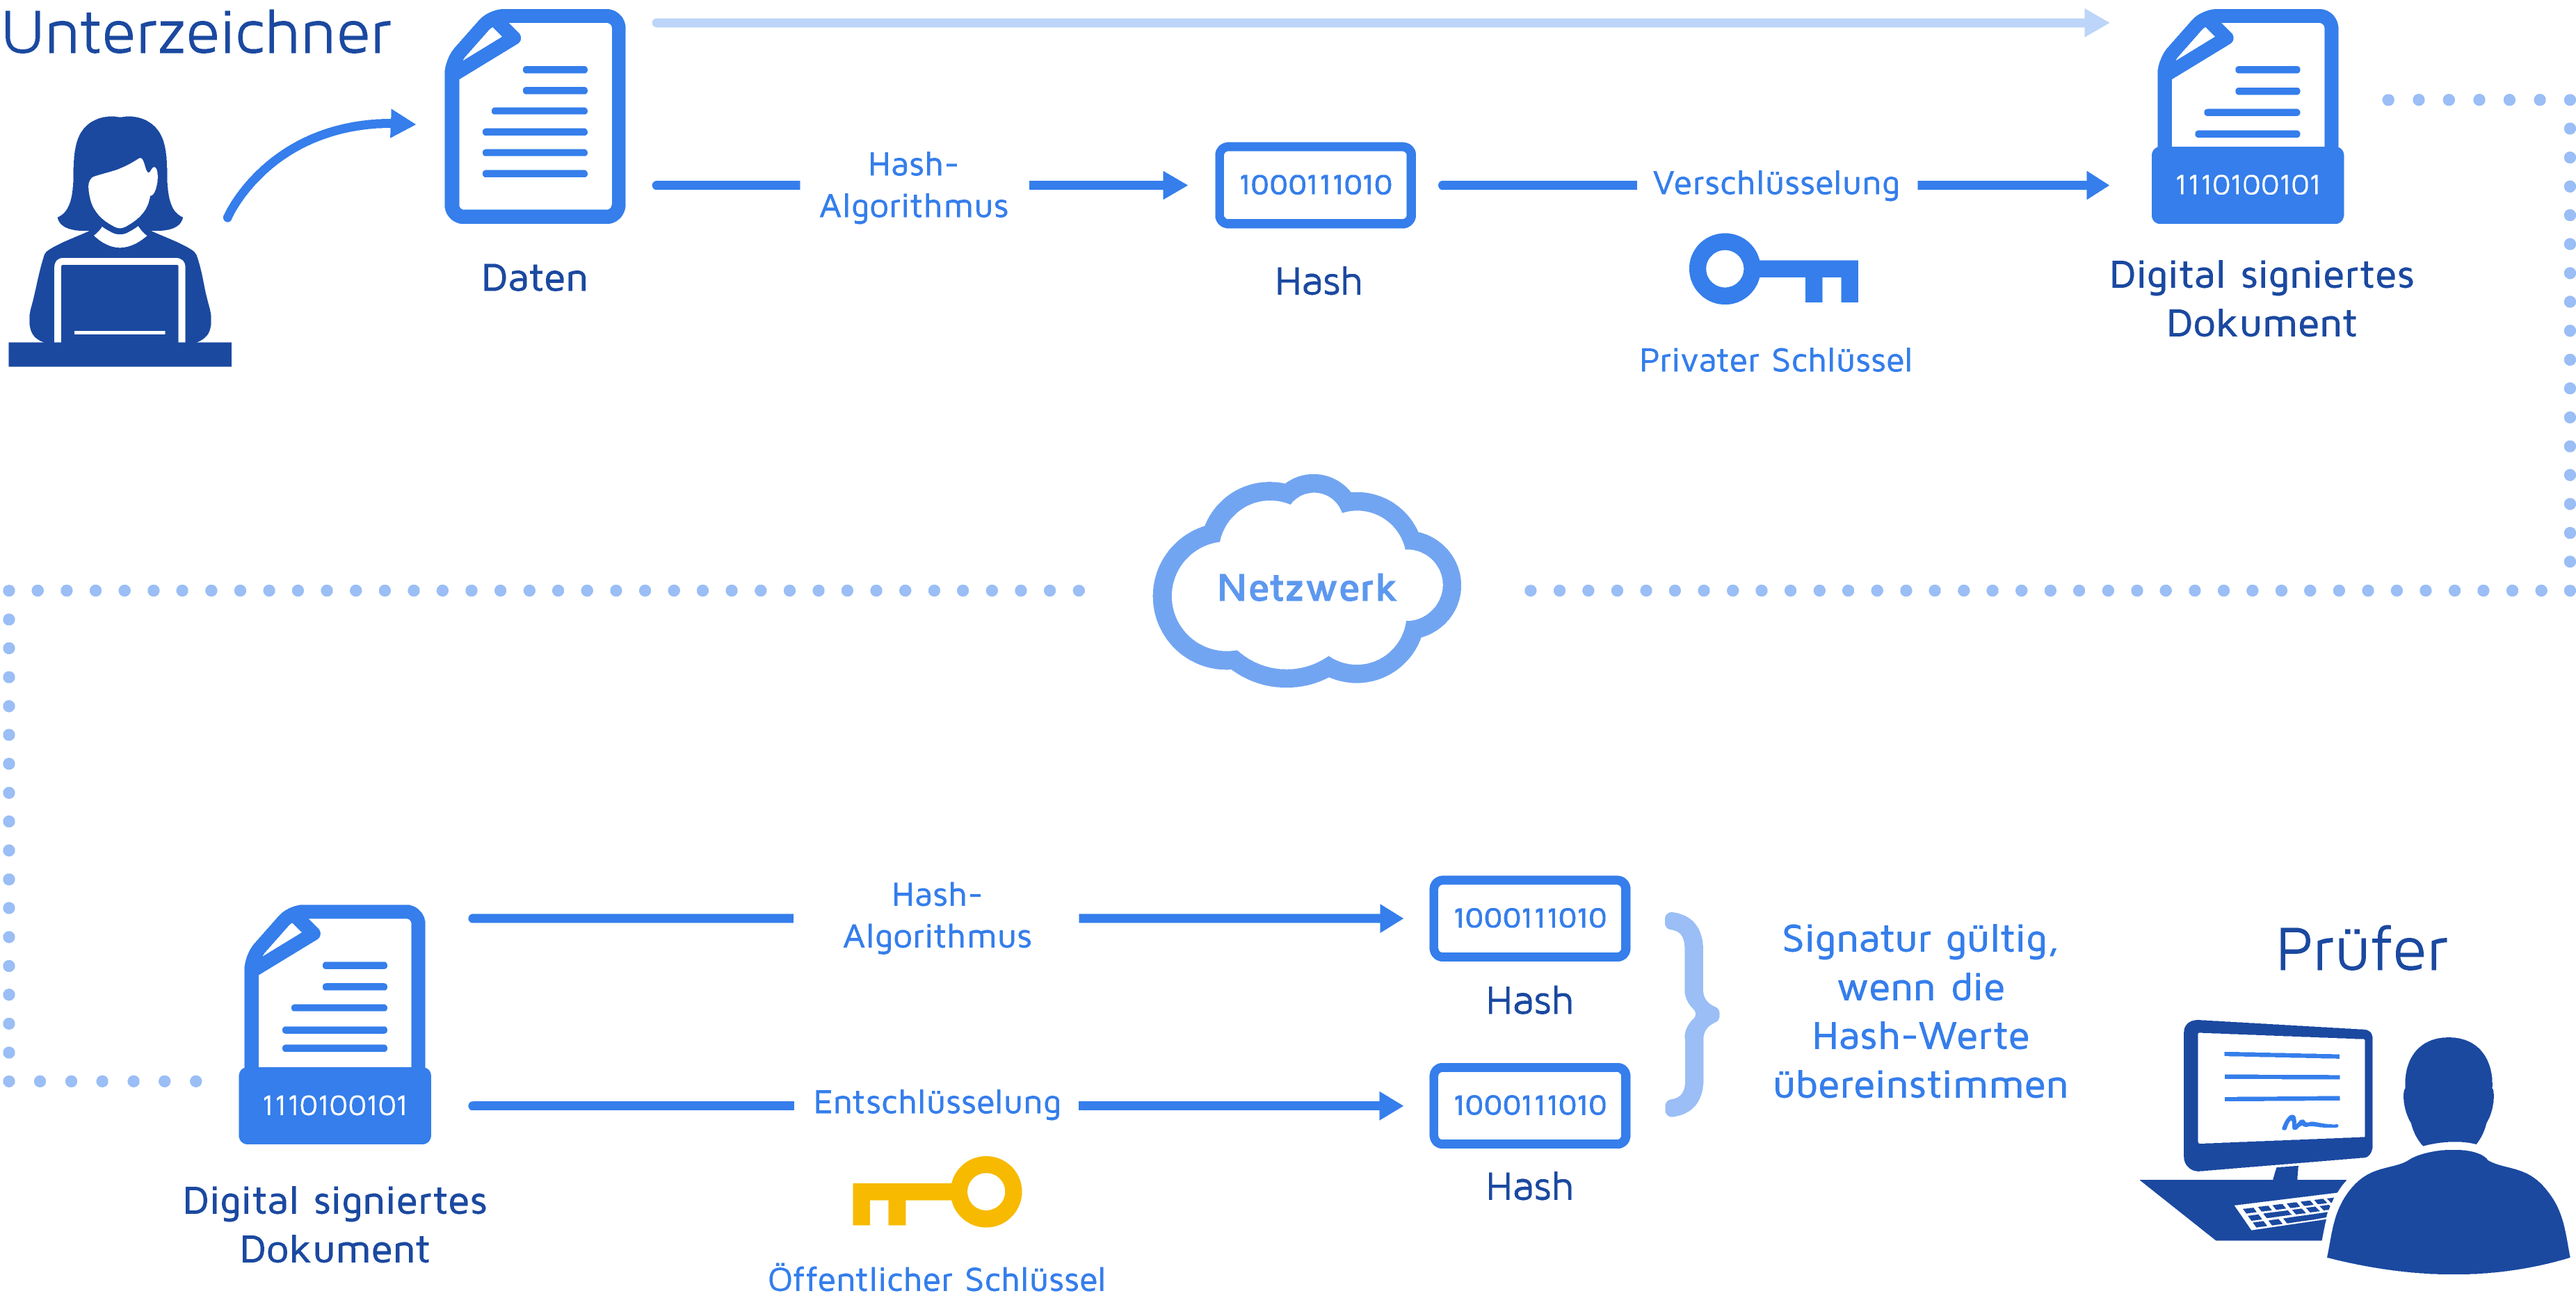
\includegraphics[scale=0.45]{Dokument_digitale_Signatur}
\caption{Abbildung zu Digitalen Signaturen}
\label{fig:figure3}
\end{figure}


Als erstes berechnet man den Hash-Wert mithilfe einer Einwegfunktion:
$$ {h = e(m)} $$

Dann berechnet man mit dem RSA-Algorithmus die Signatur \textit{s}
$$ {s = h^d \bmod n} $$

Zum überprüfen der Signatur wird erneut h bestimmt und mit dem empfangenen \textit{h} verglichen
$$ {h = s^e \bmod n} $$

Beispiel: Die digitale Signatur von \textit{m} = 8:\\ 

Angenommen:
$${ \textit{m} = 8 }$$
$${ \textit{n} = 187 }$$
$${ \textit{d} = 59 }$$
$${ \textit{e} = 19 }$$


Erst wird der Hash-Wert von \textit{m} berechnet...
$$ {16 = e(8)} $$	

...und dann mit der RSA-Funktion verschlüsselt: %richtige Formulierung?
$$ {s = 16^d \bmod n} $$	

	 	
	\subsection{Hybride Verschlüsselung}

\pagebreak
\section{Anhang}

\listoffigures
\pagebreak

\nocite{*}
\printbibliography

\end{document}
